\begin{figure}[ht!]
\center{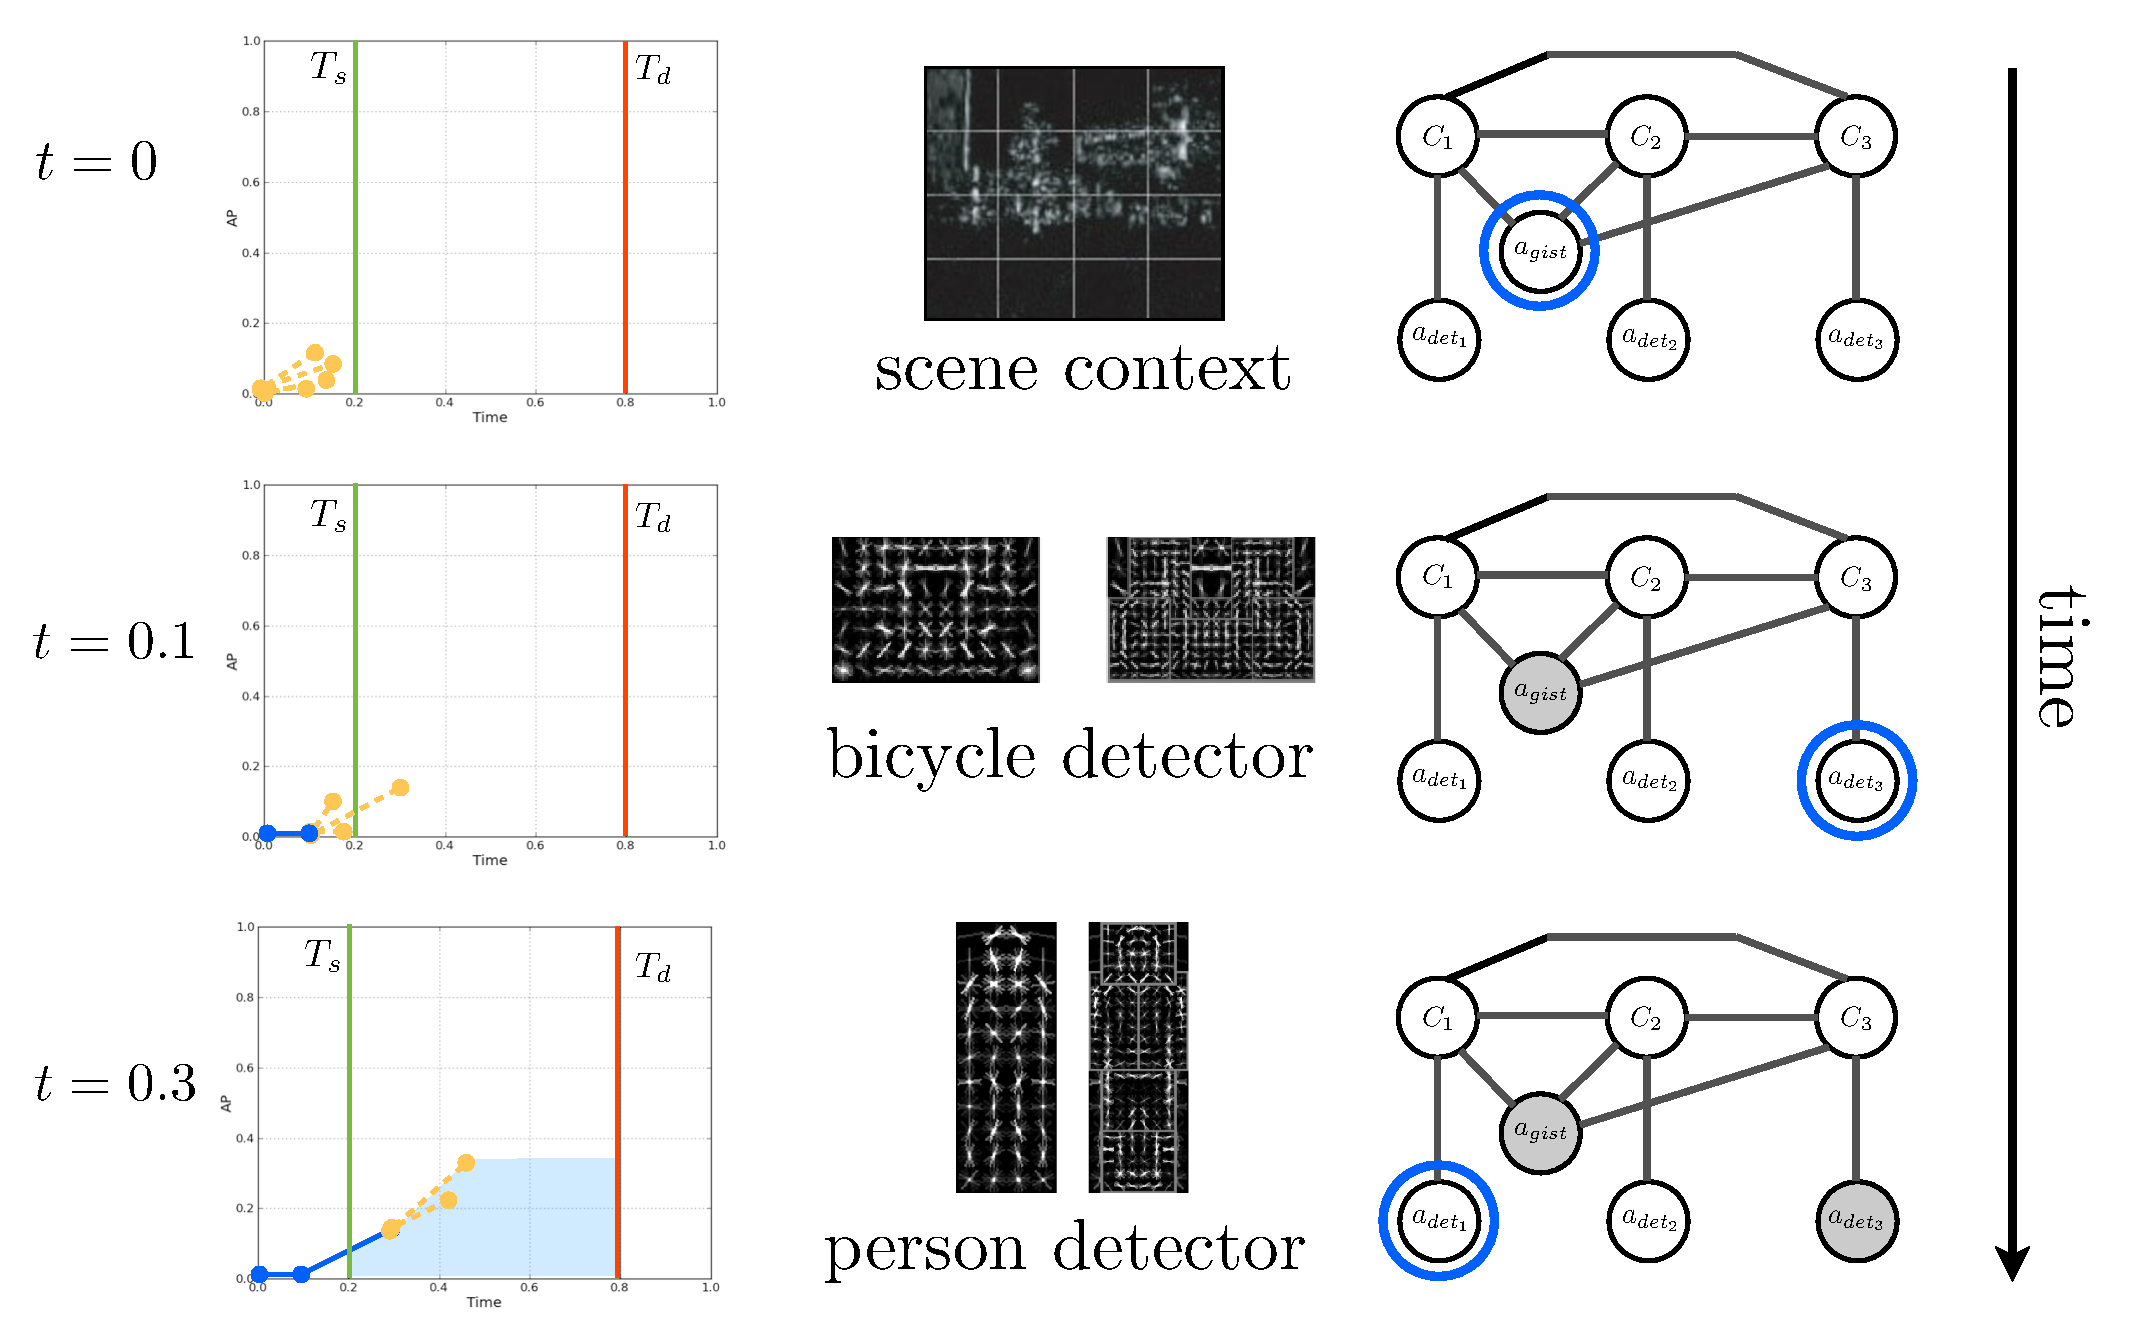
\includegraphics[width=0.86\linewidth]
    {../../../2011-2012/figures/figure1.pdf}}
  \caption{
A sample trace of our method.
At each time step beginning at $t=0$, potential actions are considered according to their predicted \emph{value}, and the maximizing action is picked.
The selected action is performed and returns \emph{observations}.
Different actions return different observations: a detector returns a list of detections, while a scene context action simply returns its computed feature.
The \emph{belief model} of our system is updated with the observations, which influences the selection of the next action.
The final evaluation of a detection episode is the area of the \emph{AP vs. Time} curve between given start and end times.
The value of an action is the expected result of final evaluation if the action is taken and the policy continues to be followed, which allows actions without an immediate benefit to be scheduled.
}\label{fig:det_figure1}
\end{figure}
